\chapter{Unit Tests}

Bei der Erstellung der Tests wurde auf die ATRIP-Regeln geachtet. Damit die Tests automatisch und wiederholbar sind, wurden sie mit xUnit erstellt und benötigen bei der Testausführung keinerlei Benutzerinteraktion. Dabei sind alle Tests unabhängig voneinander. Da sie gründlich erstellt wurden, existieren für die meisten Funktionen welche getestet werden mehrere Testfunktionen um möglichst alle Szenarien und auch Grenzfälle abzudecken. Außerdem wurde der Fokus auf Funktionen gelegt, welche für das Ausführen der Anwendung absolut notwendig sind. Dazu zählt hier vor allem das Generieren von Spielfeldern, das Auswählen von Wörtern und deren Überprüfung ob diese richtig sind.  


Die Tests wurden in der AAA-Normalform erstellt. Mock-Objekte wurden mit Moq erstellt. Ein Beispiel für die Normalform sowie die Verwendung von Mocks ist nachfolgend dargestellt. Dabei werden 5 Mocks erstellt, da diese im Konstruktor der Klasse benötigt werden und Anschließend eine Instanz der Klasse erzeugt. Danach wird die zu testende Funktion aufgerufen und anschließend überprüft ob das Ergebnis korrekt ist.

\begin{figure}[htb]
\centering
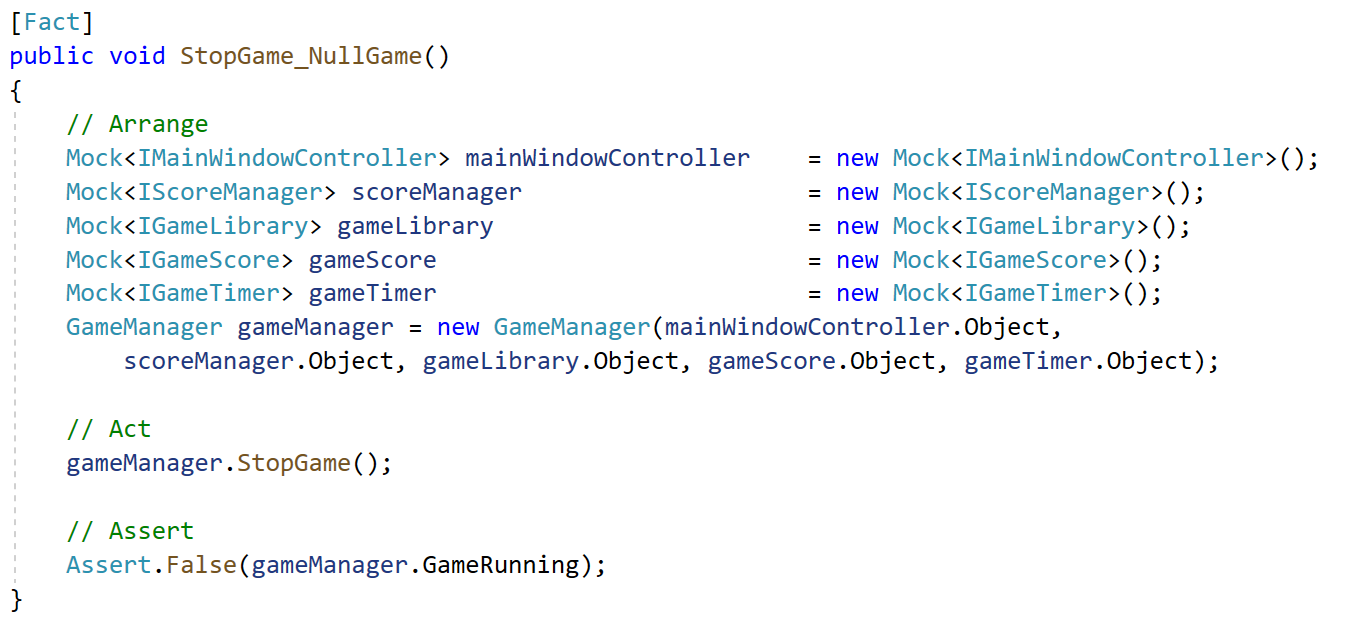
\includegraphics[width=0.7\textwidth]{Bilder/UnitTest.PNG}
\caption{\label{Abb:UnitTest}Beispiel Tests mit Mocks in AAA-Normalform}
\end{figure}



Die Testabdeckung beträgt 50\% Line Coverage.

\begin{figure}[htb]
\centering
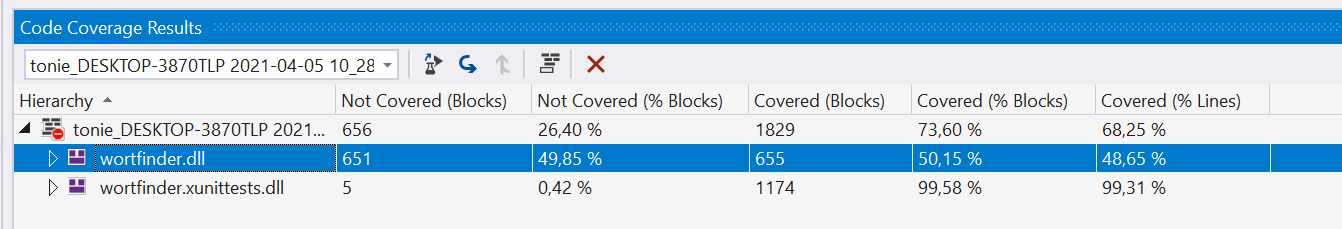
\includegraphics[width=1.0\textwidth]{Bilder/Testabdeckung.PNG}
\caption{\label{Abb:Testabdeckung}Die Ausgabe der Testabdeckung von Visual Studio}
\end{figure}

Die Abdeckung ist nicht höher, da ein Großteil der Codezeilen in den \textit{xaml} Dateien der GUI sind, welche nicht abgedeckt und nicht Unit Testbar sind. Außerdem sind primär die wichtigen Stellen im Quellcode mit Tests abgedeckt. Unwichtigere werden eher vernachlässigt.

\endinput